\newpage

\section*{\centering Author's Notes}

\begin{enumerate}
    \item If I say something is from a specific chapter, I mean that it is included in that chapter, but it isn’t necessarily the ‘whole’ chapter.
\end{enumerate}


\section*{\centering Works Cited}

Tanaka, Koji. (2004). The limit of language in Daoism. Asian Philosophy. 14. 191-205. 10.1080/0955236042000237417.

McDonald, John H. (1996). Tao Te Ching by Lao Tzu. A Modern Paraphrase.

\section*{\centering Postscript}

After reading and writing about some supposed properties of Taoism, I cannot help but remark to myself: just because something -for instance- seems bad, doesn’t make it so, if you can discern where you are in life; where clarity comes from removing oneself from the details of life.

\begin{center}
    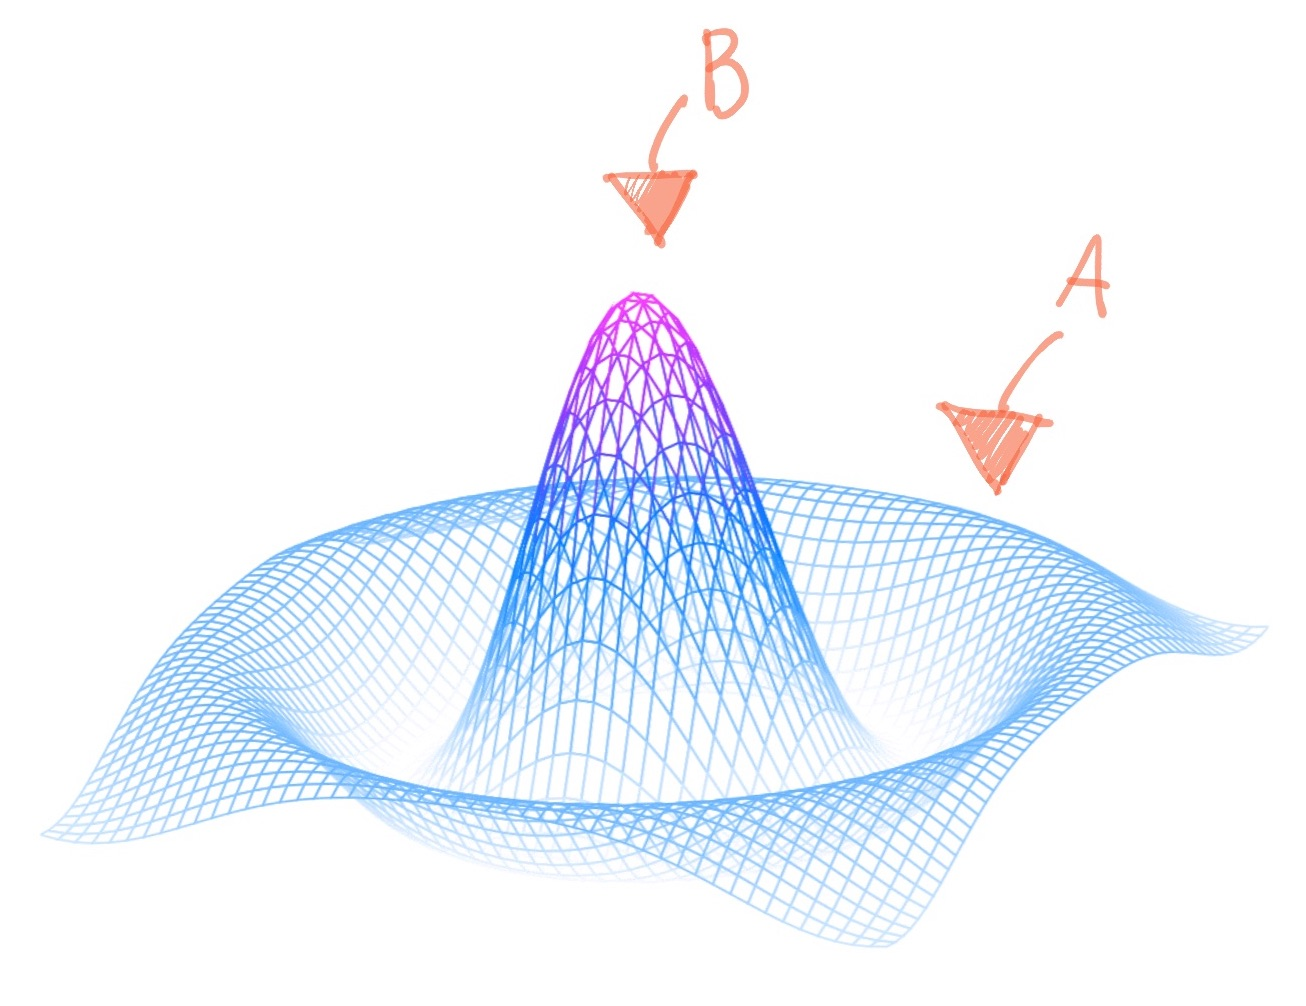
\includegraphics[width=0.9\textwidth]{../assets/image3.jpg}
    Traversing from point A to the higher point (B), requires a regression through the valley.
\end{center}

After all, the high is defined by the low, both require each other to exist, and therefore to experience the high, we must conversely experience the low, and therefore, perhaps if you can understand proportions: maybe you can see the valley for what it is, and walk through such in contentment.

